%%% Template for the submission to  %%%
%%%     Binghamton University Computer Science Department  (ndjfl)
%%%
%%% Usage summary %%%
%%%     Mostly, the information
%%%     required is obvious, but some explanations are given.
%%%     All other lines should be ignored.  

\documentclass{ndjflart}
%%% HIGHLY RECOMMENDED PACKAGES AND SETTINGS
%\usepackage{pdfsync}  %% if you know what this is use it or not. 
\usepackage[T1]{fontenc}
%%%%%%%%%%%%%%%%%%%%%%%%%%%%%%
%% If your tex system is less than 2 years old (in 2012) the following
%% font options are available. If not comment them out.
\usepackage{tgtermes}
%       otherwise use alternative journal fonts
%\renewcommand{\rmdefault}{ptm} % system default Times font
\usepackage{mathptmx}  
%%%     additional fonts
\usepackage[scaled=.92]{helvet}
%\setoptfont{enc={T1},fam={pop}} % if You have Optima font, uncomment this line
%%% MATH
\usepackage{amsthm,amsmath,amssymb}
\usepackage{mathrsfs}
%%% BIBLIOGRAPHY
\usepackage[numbers]{natbib}  %% numbers is required.
%%% LINKS
\usepackage[colorlinks,citecolor=blue,urlcolor=blue]{hyperref}  %%check
\usepackage{graphicx}

\artstatus{am} %%% leave this alone!!  That means you, too!!
%%%%%%%%theorems%%%%%


%%%% feel free to changes these%%%%%%%
\newtheorem{theorem}{Theorem}[section]
\newtheorem{lemma}[theorem]{Lemma}
\newtheorem{conjecture}[theorem]{Conjecture}
\newtheorem{condition}[theorem]{Condition}
\newtheorem{claim}[theorem]{Claim}
\newtheorem{question}[theorem]{Question}
\newtheorem{corollary}[theorem]{Corollary} 
\theoremstyle{definition}
\newtheorem{definition}[theorem]{Definition}
\newtheorem{statement}[theorem]{Statement}
\newtheorem{notation}[theorem]{Notation} 
\theoremstyle{remark}
\newtheorem{remark}[theorem]{Remark}



%%%DATE enter the date of your submission here- best%%%
%%%If \date{} is not used, the current date will be used%%%
%%%Warning:This will be lost if your paper is recompiled on another day though%%%
%%%\date{May 30, 2012}%%%%
\date{December 12, 2019}

%%%PUT YOUR DEFINITIONS HERE%%%
%NDJFL uses \varphi by default; redefine only if you want \phi%%%

\startlocaldefs
%%% our macros for this article only %%%%
\newcommand{\NDJFL}{\emph{NDJFL}}
\newcommand{\Jo}{\emph{Journal}}
\newcommand{\EM}{Editorial Manager}
\newcommand{\origphi}{\phi}
\newcommand{\CMS}{\emph{CMS}}
\newcommand{\mn}{\medskip\noindent}
\newcommand{\tietilde}{\char126\relax}

\endlocaldefs

\begin{document}

\begin{frontmatter}

  %% TITLE OF YOUR PAPER%%%
  %% Words in title should begin with uppercase, except%%%
  %%% articles (and, the, a), conjunctions (and, for, nor, but),
  %%% prepositions (by, with, for, over, and so on)
  \title{\emph{Development of Human Following}\\
    \emph{Mobile Robot System}}
  %%% Choose a short title to be used as the running head on
  %%% odd-numbered pages%%%
  %%% Use this same title as "short title" when you submit MS to
  %%% EM%%%%
  \runtitle{Development of Human Following Mobile Robot System}

  \author{\fnms{Umut} %first name
    \snm{Kayaalti}%last name
    \corref{}%to denote who is the corresponding author
    \ead[label=e1]{ukayaal1@binghamton.edu}%author email, leave this [label] as is
    \ead[label=u1,url]{}%%web page, leave this [label] as is
  }
  %%% ADDRESS NOTES
  %%% Dept listed first, University/company second, street or PO box
  %%% third%%%
  %%% U.S. Postal Service guidelines request no punctuation in the
  %%% street...country lines%%%
  %%% Country should be all uppercase%%%%
  \address{Thomas J. Watson School of Engineering\\
    Binghamton University\\
    4400 Vestal Parkway East\\
    Binghamton NY 13902\\
    USA\\
    \printead{e1}\\
    \printead{u1} }%
  \and%
  \author{\fnms{Emily}
    \snm{Lakic}\ead[label=e2]{elakic1@binghamton.edu}}%increase label by
  %	% one for each
  %	% author
  \address{Thomas J. Watson School of Engineering\\
    Binghamton University\\
    4400 Vestal Parkway East\\
    Binghamton NY 13902\\
    USA\\
    \printead{e2} }
  % \and \author{\fnms{???} \snm{???}\ead[label=e3]{???}}
  % \address{\printead{e3}} \affiliation{???}

  %%%% INSERT EACH AUTHOR'S FIRST INITIAL AND SURNAME%%%%
  \runauthor{U.~Kayaalti and E.~Lakic}


\begin{abstract}
A human-following robot has plenty of applications in daily life and manufacturing. Autonomous robots can learn to 'follow the leader' in an effort to provide as mission partners for humans, whether to assist in day-by-day tasks or for more extensive use as industrial robots operating in complex environments. The purpose of the development of a human following mobile robot system is to provide a robot the ability to actively follow a person while keeping a certain distance. If that person moves away, the robot will move until the person is as close as the specified distance again, or will rotate to keep him/her in its lenses. Robotic vision tools will operate vastly from the generation of robot movement through the integration of the PointCloud algorithm for motion analysis, to  the use of rapid RGB image processing and open source computer vision libraries to detect human activity. A more complex analysis of the distance between the robot and said human will be measured by a ros scan as well as setting a specific goal distance between the two respective objects at play.
\end{abstract}

\begin{keyword}[class=AMS]
  \kwd[Primary ]{X001} \kwd{Y002} \kwd[; Secondary ]{Z003}
\end{keyword}

\begin{keyword}
  \kwd{Faster R-CNN} \kwd{RPN} \kwd{PointCloud} \kwd{TurtleBot}
\end{keyword}

\end{frontmatter}

% main matter with bibliography goes here

\section{Problem to Solve}\label{intro}
The use of artificial intelligent robotic systems in correspondence to human-following has potential uses from simple tasks of accompanying an owner and helping an elderly with their daily tasks, to taking care of children and aiding in military, espionage, and information gathering. Societal needs in such modern times demand for human detection and following systems to be implemented as modernized innovations in technology, such as self-driving cars, do and will in future times require the issue at hand to be solved. Development in hardware - especially modern graphics processing units - along with that of modern efficient algorithms and large sets of data for training these algorithms, all provide leeway into the emphasis of finding a solution in our present day.

\begin{figure}
\begin{center}
\vspace{0.5em}
    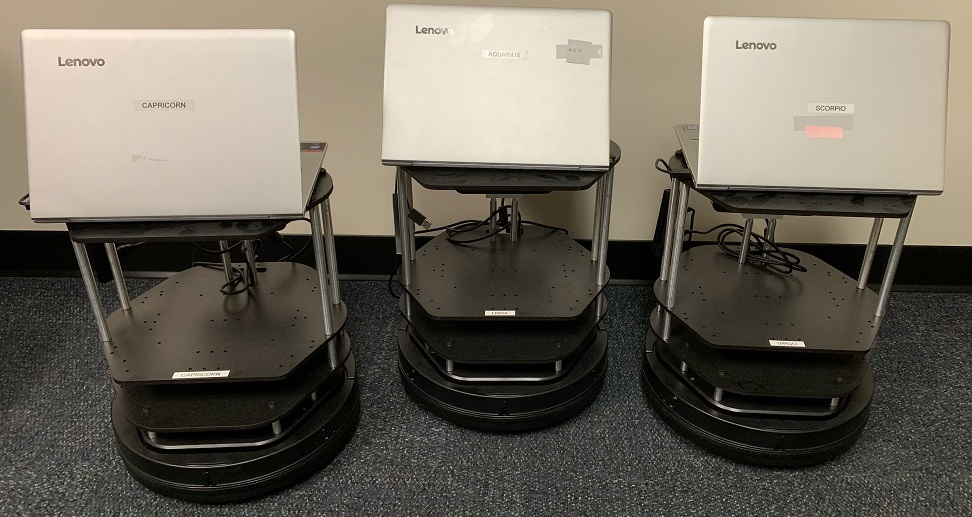
\includegraphics[width=8cm]{images/turtlebots}
    \vspace{-.5em}
\caption{TurtleBots used for testing purposes. }
\label{fig:framework}
    \end{center}
\end{figure}

\section{Literature}\label{front}
Past research done on human detection and following systems gave insight into relevant methods to approaching the objectives at hand. Both object detection and robot movement were studied extensively prior as a means to assemble a thorough plan of action when considering the two processes functioning as one.

\begin{figure}
\begin{center}
\vspace{0.5em}
    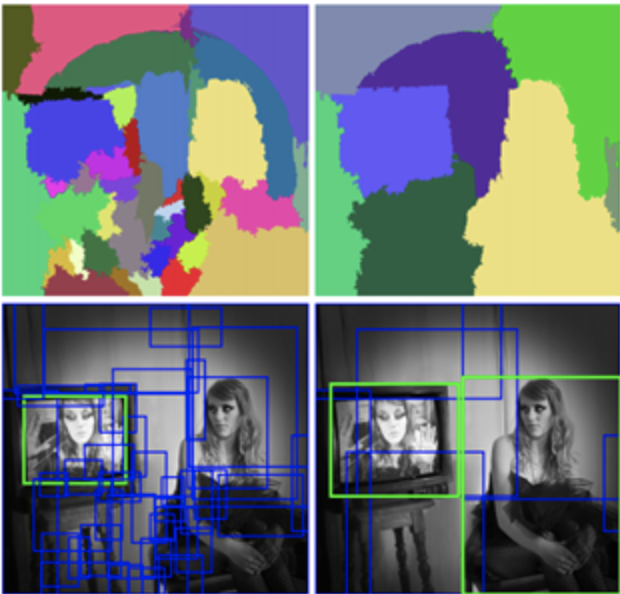
\includegraphics[width=8cm]{images/detection}
    \vspace{-.5em}
\caption{Selective Search Algorithm for Detection. }
\label{fig:framework}
    \end{center}
\end{figure}

\subsection{Object Detection}\label{fonts} 
%
Object detection algorithm is used to get the information of which objects are inside of the image, it also puts boxes to indicate where the objects are residing in the image. It takes a whole image as its input and returns the which class they belong to with the probability of the objects existing in that image. For example, a class label could be “dog” and the associated class probability could be 97 percent. For localizing where the object is, we must inspect sub-regions or patches of the image and then apply the object detection network or the classifier to these image patches. The simplest method for creating smaller sub-regions or patches is called the Sliding Window approach. This method works by iterating over the entire image with different sized rectangles and inspecting those smaller images in a brute-force-method. Unfortunately, you will have a huge number of smaller images to look at. These constraints are triumphed by the “Region Proposal” algorithms such as Selective Search algorithm, as shown in Figure 2. Region Proposal Algorithms work by taking an image as the input and putting boxes on all patches that has a high probability of containing an object. These region proposals have high false positive by intention so that even though these overlapping regions may not encompass the entire object one of these boxes will contain a good portion of the object that will get a true positive from the classification algorithm. Region proposal algorithms identify objects in an image using segmentation [3]. In segmentation, we group adjacent regions which are similar to each other based on some criteria such as color, texture, etc. Unlike the sliding window approach where we are looking for the object at all pixel locations and at all scales, region proposal algorithm works by grouping pixels into a smaller number of segments. 

\begin{figure}
\begin{center}
\vspace{0.5em}
    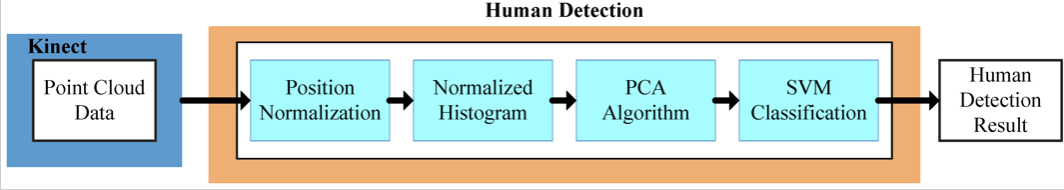
\includegraphics[width=8cm]{images/pointcloud2}
    \vspace{-.5em}
\caption{Point Cloud Integration to Human Detection and Following. }
\label{fig:framework}
    \end{center}
\end{figure}

\subsection{Robot Movement}\label{macros} 
The PointCloud library is the most common point cloud processing framework in ROS, and for the purposes of this project, served to accurately assist in robot movement while following a human detection algorithm. An RGBD image combining images from the robot's depth and RGB camera provided a list of points, with each point representing an xyz position within the point cloud. The PointCloud library filters point clouds using a cropping mechanism. Camera coordinates of the depth and RGB cameras yield dimensions of a box that the PointCloud library searches for a human in. In this system, the x-coordinate is represented by the left/right motion, the y-coordinate is represented by the up/down motion, and the depth is measured by the forward and backward movements and represented by the z-coordinate. Past research uses a variety of formulas to grab point cloud data from the environment and normalize it based on the point cloud position of each of the three coordinates x, y, and z, as shown in Figure 3. These formulas are as follows: \textit{xdiff = xmax - xmin}, \textit{ydiff = ymax - ymin}, and \textit{zdiff = zmax - zmin}. A normalized histogram is composed to reduce the dimensions of the box that the PointCloud library uses for detection and retrieving any associated points. A support vector machine predictor further classifies human and non-human classes with respect to the input point cloud data.

\section{Technical Details}\label{secs} 

\subsection{Faster-RCNN}\label{ssecacks}
The algorithm that Umut used for detection is a variant of R-CNN called Faster R-CNN. Faster R-CNN is a network that does object detection and compared to previous work, Faster R-CNN employs a region proposal network which is a separate network and does not require an external method for candidate region proposals, as shown in Figure 4.  
\begin{figure}
\begin{center}
\vspace{0.5em}
    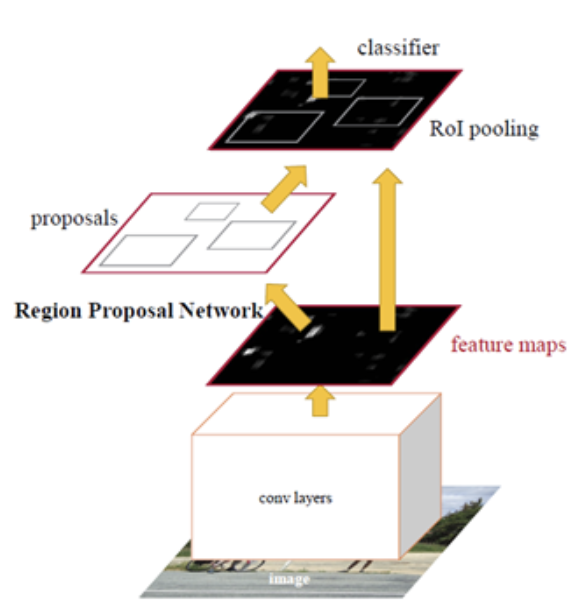
\includegraphics[width=8cm]{images/fasterrcnn}
    \vspace{-.5em}
\caption{Faster R-CNN. }
\label{fig:framework}
    \end{center}
\end{figure}

\begin{figure}
\begin{center}
\vspace{0.5em}
    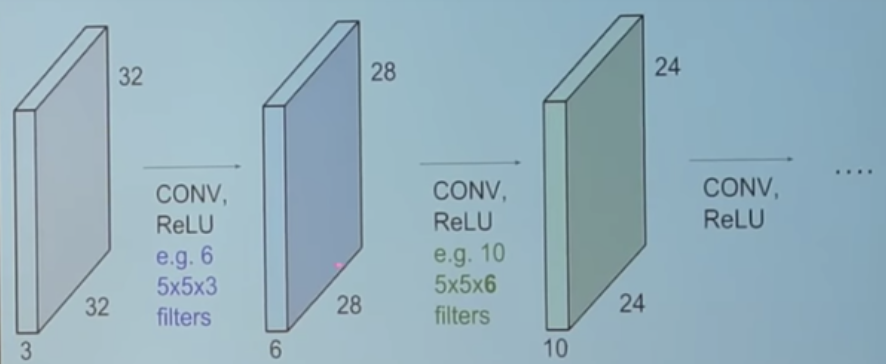
\includegraphics[width=8cm]{images/CNN}
    \vspace{-.5em}
\caption{CNN. }
\label{fig:framework}
    \end{center}
\end{figure}

\subsection{CNN}\label{ssecnotes}
The algorithm first runs the image through a CNN to get Feature maps extracted. To get a single feature map we run a filter represented by a matrix of weights with which we convolve with the input. Features maps are a representation of the dominant features of the image at different scales, as shown in Figure 5. By applying several convolutions and pooling layers in a row output features are much smaller than the input image. For every point in the output feature map, the region proposal network has to learn whether an object is present in the input image at that coordinates and determine its size. This part is done by placing a set of “Anchors” on the input image for each location on the output feature map. These anchors indicate possible objects in various sizes and aspect ratios at this location.

\begin{figure}
\begin{center}
\vspace{0.5em}
    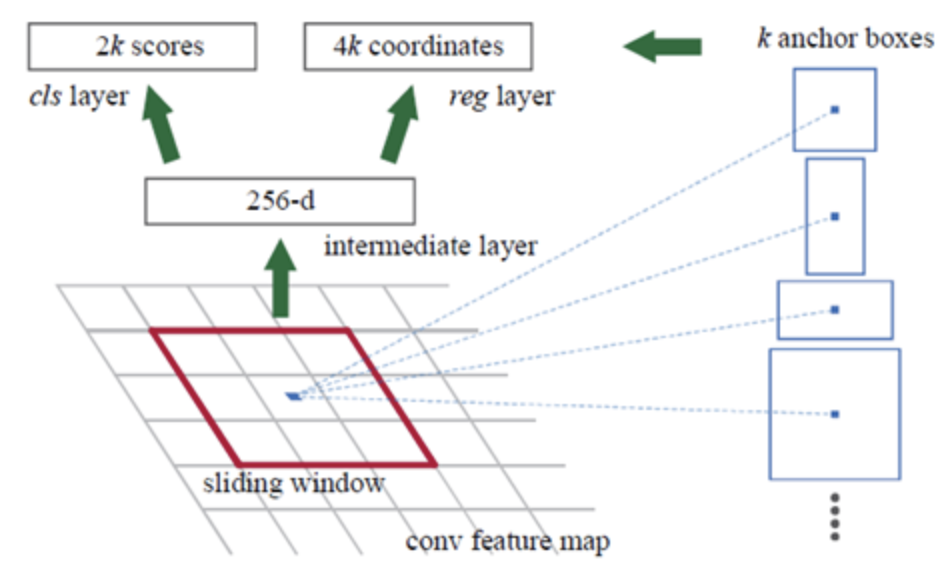
\includegraphics[width=8cm]{images/RPN}
    \vspace{-.5em}
\caption{RPN. }
\label{fig:framework}
    \end{center}
\end{figure}

\subsection{RPN}\label{ssecnotes}
Region Proposal Network iterates through each point in the output feature map, it has to check whether these k corresponding anchors placed in the input image actually contain objects and refine these anchors’ coordinates to give bounding boxes as “Object proposals” or regions of interest, as shown in Figure 6. The cls layer of the network outputs 2 scores for each k anchor boxes for the one for the possibility of it containing an object and one for the possibility of not containing an object.
The reg layer outputs 4 coordinates (x,y, width and height) for each k anchor boxes. These regression outputs are used on improving the coordinates of the anchors that contain objects.
With a size of Width × Height of feature map, there will be Width × Height × k anchors in total.
Using the predictions from RPN, we pick the top anchors that has the highest likelihood of containing objects and refine their location and size. If there are good anchors that are overlapping too much, we keep the one with the highest foreground (an object and not background) score and discard the rest which is named as Non-max Suppression. Finally, we have the final proposals that we can pass to the next stage.

\begin{figure}
\begin{center}
\vspace{0.5em}
    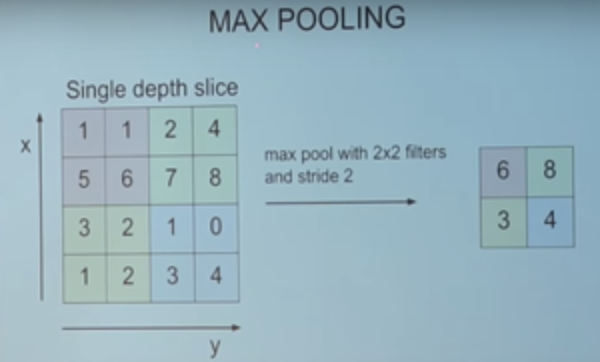
\includegraphics[width=8cm]{images/maxpooling}
    \vspace{-.5em}
\caption{Max Pooling. }
\label{fig:framework}
    \end{center}
\end{figure}

\subsection{Detection Network}\label{ssecnotes}
Proposals gained from the RPN are used for pooling features from the original feature map. This is done by the Region of Interest pooling layer, as shown in Figure 7. ROI pooling layer works by taking the region corresponding to a proposal from the original feature map. Afterwards ROI pooling layer divides this region into a fixed number of sub-windows. Finally, by performing max pooling over these sub-windows to give a fixed size output. Max pooling works by taking the biggest input from the corresponding subdivision to represent that entire subdivision. The output features from the ROI Pooling layer are fed into the sibling classification and regression layers. Classification network has one output for each class. These classification scores represent the likelihood of belonging to each class, including a catch-all background class. The features in the end of the classification passed through a softmax layer which is a type of squashing function that limits the output of the function into the range 0 to 1 to get the classification scores. The regression layer coefficients are used to improve the predicted bounding boxes for each class. All the classes have individual regressors with 4 parameters each corresponding to class*4 output units in the regression layer.

\subsection{PointCloud}\label{ssecnotes}
Following the implementation of human detection algorithms to accurately locate a human's figure, more precisely their lower body, the Point Cloud algorithm analyzed dimensions of the box detecting a human figure to precisely assign camera coordinates in x, y, z values. Important prior to implementation is ensuring a robot does not approach a human too close. In an effort to avoid collision, a goal distance measured by the depth coordinate z would set an appropriate distance between the robot and human while applying a depth threshold to inform the robot on how far away from the distance it is before it reacts. Maximum and minimum linear and angular speeds, as well as a publisher and subscriber, were implemented to control the robot's movement. Centroid coordinates were initialized to a specific point count prior to reading in the xyz coordinates of any points provided by the cloud. If points were detected by the point cloud, centroid coordinates were computed. As our robot frequently turned far right upon detecting a human and following it, we implemented two if statements to assist the robot in its left linear movement. Ensuring the maximum and minimum specifications defined prior were met, and our movement thresholds were correct by computing the linear and angular components of the movement, the robot movement command was published. 

\section{Success Criteria}\label{ams}
The robot was detecting the human accurately from the lower angle astra camera just by the combination of legs and feet. After detection it was successfully able to keep the detected human in its sights by combinations of rotations and angular movements. Using the depth view from astra robot was able to successfully calculate its distance from the human and if it was above a certain threshold robot would move towards the human to keep them in a certain distance by a combination of linear and angular movements. PointCloud calculations worked accurately following that centroid coordinates were calculated for any number of points received in the dimensions of the boxes surrounding the human's legs and feet, ensuring proper movement thresholds and meeting our maximum and minimum specifications for angular and linear speed. There were unfortunately significant lag problems due to processing power required for the human detection. This lag caused robot to lag in real time. To counter this, we had to slow down the speed of robot significantly which in turn made the testing robot harder and much less applicable to real life human tracking.

\section{Distribution}\label{refs} 

Umut has worked on the vision part of the project. He used the TensorFlow’s Object Detection API as a base to run the models pre-trained on COCO Dataset from TensorFlow Detection Model Zoo. He tried different vision-based approaches for human detection ranging from R-CNN to Single Shot Detector but finally settled on the Faster-RCNN. Emily has worked on the robot movement part of the project. She used the Point Cloud Library ROS Interface Stack. Given the project handled both 3D geometry processing in ROS as well as n-D Point Clouds for application purposes, the PointCloud package provided a significant bridge between the two. Lastly, Emily and Umut worked together on combining the vision with the movement on the TurtleBots shown in Figure 1.


\section{Conclusion}\label{whitesp}

In this project, we have described a human-following mobile robot system. One of the main conclusions Umut has arrived at is how limiting hardware and algorithms can be for real time application. Running a few of the algorithms for human detection made me realize how hard its to balance between accuracy and speed. It was clear that there are no clearly better, one size fits it all algorithm and trial and experimenting was absolutely necessary. He also had to face that no matter how suited the algorithm of choice for the task at hand was, hardware still could bottleneck the whole process. One of the main conclusions Emily arrived at from this project is that experimentation is key to achieving a functional system. This served as a technical lesson for her; different combinations of values for the maximum and minimum linear and angular speeds played a significant role in how capable the robot was when turning left and/or right while accurately following the human. 

\begin{thebibliography}{5}
\expandafter\ifx\csname natexlab\endcsname\relax\def\natexlab#1{#1}\fi
\def\docolon{:}
\def\eatcomma#1{}
\def\onlyone#1{\gdef\oneletter{#1}}
\def\sphref#1#2{{\let\#=\docolon\xdef\one{#1}}\href{\one}{#2}}
\def\zhref#1,#2{{\let\#=\docolon\xdef\one{#1}}\href{\one}{#2}}
\expandafter\ifx\csname url\endcsname\relax
  \def\url#1{{\tt #1}}\fi
\newcommand{\enquote}[2]{``#1,''}

\bibitem[Ren(2016)]{ant10}
Ren, S.,
\newblock \enquote{Faster R-CNN: Towards Real-Time Object Detection with Region Proposal Networks}, {\em Cornell University}, (2016),
  \sphref{https://arxiv.org/abs/1506.01497}{\hbox{MR 2667904}}.

\bibitem[Zhao(2019)]{copy}
Zhao, Z.,
\newblock \enquote{Object Detection with Deep Learning: A Review},
\newblock Cornell University, Ithaca, 2019.

\bibitem[Clemens(2009)]{cle09}
Uijlings, J.~R.~R.,
\newblock \enquote{Selective Search for Object Recognition},
\newblock {\em University of Trento, Italy}, (2012),
  pp.~1--14.\eatcomma. \zhref{https://ivi.fnwi.uva.nl/isis/publications/2013/UijlingsIJCV2013/UijlingsIJCV2013.pdf},
  {\hbox{Zbl 1188.03031}}.
  \sphref{http://www.ams.org/mathscinet-getitem?mr=2536697}{\hbox{MR 2536697}}.

\bibitem[Girshick(2015)]{ghma09}
Girshick, R. \unskip,
``Fast R-CNN''
{\em Microsoft Research}, (2015),
  pp.~1--9.\eatcomma.
  \zhref{https://arxiv.org/pdf/1504.08083.pdf}, {\hbox{Zbl
  1223.03052}}.
  \sphref{http://www.ams.org/mathscinet-getitem?mr=2598871}{\hbox{MR 2598871}}.

\bibitem[Jerbić(2015)]{CMS} Jerbić, B.,
\newblock \enquote{Robot Assisted 3D Point Cloud Object Registration}, vol. 100 (2015),
\newblock Procedia Engineering, Zagreb, Croatia 2015.

\bibitem[Miao(2016)]{CMS} Miao, Y.,
\newblock \enquote{The Pose Estimation of Mobile Robot Based on Improved Point Cloud Registration}, vol. 100 (2016),
\newblock International Journal of Advanced Robotic Systems, Xuzhou City, China 2016.

\bibitem[Saputra(2018)]{CMS} Saputra, R.,
\newblock \enquote{Casualty Detection from 3D Point Cloud Data for Autonomous Ground Mobile Rescue Robots}, (2018), pp.~1--7.
\newblock IEEE International Symposium on Safety, Security, and Rescue Robotics, Philadelphia, PA 2018.

\end{thebibliography}


%\bibliographystyle{jflnat} 
%\bibliography{GTA}

%%% ACKNOWLEDGMENTS= your personal comments and thanks %%%
\begin{acks}
  We are grateful to Professor Shiqi Zhang of Binghamton University’s Computer Science Department. We are thankful for the robot use provided by both Professor’s Lab as well as Binghamton University’s Lab.

\end{acks}

\end{document}


%%%%%%%%%%%%%GTA.bib%%%%%%%%%%
@book{CMS,
	EDITOR = {University of Chicago Press Staff},
	TITLE = {The Chicago Manual of Style},
	PUBLISHER = {The University of Chicago Press},
	ADDRESS = {Chicago},
	YEAR  = {2010},
	EDITION = {16th}
}

@book{copy,
	TITLE = {Butcher's {C}opyediting: {T}he {C}ambridge {H}andbook for {E}ditors, {C}opyeditors and {P}roofreaders},
	AUTHOR = {Judith Butcher},
	PUBLISHER = {Cambridge University Press},
	ADDRESS = {Cambridge},
	YEAR = {1981},
	EDITION = {4th}
}

@article{ghma09,
	AUTHOR = {Gherardi, Guido and Marcone, Alberto},
	TITLE = {How incomputable is the separable {H}ahn-{B}anach theorem?},
	JOURNAL = {Binghamton University Computer Science Department},
	VOLUME = {50},
	YEAR = {2009},
	NUMBER = {4},
	PAGES = {393--425},
	ISSN = {0029-4527},
	MRCLASS = {03F60 (03B30 46A22 46S30)},
	MRNUMBER = {2598871},
	MRREVIEWER = {Klaus Weihrauch},
	ZBLNUMBER = {1223.03052}
}
       
@article{ant10,
	AUTHOR = {Antonelli, G. Aldo},
	TITLE = {Numerical abstraction via the {F}rege quantifier},
	JOURNAL = {Binghamton University Computer Science Department},
	VOLUME = {51},
	YEAR = {2010},
	NUMBER = {2},
	PAGES = {161--179},
	ISSN = {0029-4527},
	MRCLASS = {03C80},
	MRNUMBER = {2667904},
	ZBLNUMBER = {1205.03055}
}

@article{cle09,
	AUTHOR = {Clemens, John D.},
	TITLE = {Isomorphism of homogeneous structures},
	JOURNAL = {Binghamton University Computer Science Department},
	VOLUME = {50},
	YEAR = {2009},
	NUMBER = {1},
	PAGES = {1--22},
	ISSN = {0029-4527},
	MRCLASS = {03E15 (03C15 03C50)},
	MRNUMBER = {2536697},
	MRREVIEWER = {Barbara Majcher-Iwanow},
       ZBLNUMBER = {1188.03031}
}
